\documentclass[aspectratio=169,
				xcolor=table]{beamer}

% Load general definitions
\usepackage[utf8]{inputenc}
%\usepackage[T1]{fontenc}
\usepackage[brazil]{babel}
\usepackage{amsmath}
\usepackage{amsfonts}
\usepackage{amssymb}
\usepackage{graphicx}
\usepackage{verbatim}
\usepackage{cancel}
\usepackage{askmaps}
\usepackage{tabularx}
\usepackage[table]{xcolor}
%\usepackage{tikz}
\usepackage{multirow}
\usepackage{mathtools}
\usepackage{color, colortbl}
\usepackage{etoolbox}
\usepackage{pbox}
\usepackage{changepage}
\usepackage{xpatch}
\usepackage{array}
\usepackage{marvosym}
\usepackage{tabu}
\usepackage{multicol}
\usepackage{listings}
\usepackage{underscore}
\usepackage{filecontents}
\usepackage[]{algorithm2e}
\usepackage{ragged2e}

\newcolumntype{P}[1]{>{\centering\arraybackslash}m{#1}}
\definecolor{Gray}{gray}{0.75}
\definecolor{Gray2}{gray}{0.85}

\definecolor{lightBlue}{HTML}{DAE8FC}
\definecolor{Blue}{RGB}{51, 51, 204}

%\useinnertheme[lily]{rounded}
\usetheme{UniEvangelica}
%\usetheme{Copenhagen}
%\usetheme{Berlin}
%\usecolortheme{dolphin}
\tolerance=1
\emergencystretch=\maxdimen
\hyphenpenalty=10000
\hbadness=10000

\setbeamertemplate{navigation symbols}{}%remove navigation symbols


\let\olditem=\item% 
\renewcommand{\item}{\olditem \justifying}%
\def\center{\trivlist \centering\item\relax}
\def\endcenter{\endtrivlist}

\setbeamertemplate{itemize/enumerate body begin}{\large}
\setbeamertemplate{itemize/enumerate subbody begin}{\large}

\setbeamertemplate{itemize item}{\raisebox{0.1ex}{$\blacktriangleright$}\hskip0.1em}
\setbeamertemplate{itemize subitem}{\raisebox{0.1ex}{$\blacktriangleright$}\hskip0.1em}

\newcommand{\greenarrow}{\textcolor{green}{\rotatebox[origin=c]{180}{\MVArrowDown}}}

\newcommand{\redarrow}{\textcolor{red}{\MVArrowDown}}

%\newcommand{\ftable}{
%	\begin{table}
%		\large
%		\centering
%		\rowcolors{1}{\ifnumless{\rownum}{2}{Blue}{lightBlue}}{}
%}

\newenvironment{eftable}{
	\begin{table}
		\large
		\centering
		\rowcolors{1}{}{Blue}
		\rowcolors{1}{\ifnumless{\rownum}{2}{Blue}{lightBlue}}{}
	}
	{
	\end{table}
}


%\setbeamertemplate{frametitle}
%{
%	%\vspace*{-2em}	
%	\insertframetitle
%
%	 %\textcolor{white}{\LARGE \insertframetitle}
%
%}

% Specific definitions
\institute[]{\uppercase{Engenharia de Software}}
\title[]{Sistemas Distribuídos}
\subtitle[]{\uppercase{Modelos Fundamentais}}
\author[]{Prof. M.e Alexandre Tannus}
\date{Anápolis - 2021.1}

%\AtBeginSection{\frame{\tableofcontents[currentsection]}}

\begin{document}
	\begin{frame}
		\titlepage		
	\end{frame}

	\begin{frame}
		\tableofcontents
	\end{frame}	

	\section{Introdução}
	\begin{frame}
		\frametitle{Introdução}
		\begin{itemize}
			\item Modelos
			\begin{itemize}
				\item Explicitam informações necessárias e relevantes sobre o sistema
				\item Tratam as possibilidades e impossibilidades de acordos com as informações disponíveis
				\begin{itemize}
					\item Algoritmos de propósito geral
					\item Propriedades  desejáveis
				\end{itemize}
			\end{itemize}
		\end{itemize}		
	\end{frame}

	\begin{frame}{Modelos Fundamentais}
		\begin{itemize}
			\item Interação
			\begin{itemize}
				\item Atrasos de comunicação
				\item Coordenação de processos
				\item Tempo global
			\end{itemize}
			\vspace{0.7em}
			\item Falha
			\begin{itemize}
				\item Máquinas
				\item Redes
			\end{itemize}
			\vspace{0.7em}
			\item Segurança
			\begin{itemize}
				\item Ataques externos e internos
				\item Define e classifica formas de ataque
			\end{itemize}
		\end{itemize}
	\end{frame}
	
	\section{Modelo de Interação}	
	\begin{frame}{Modelo de Interação}
		\begin{itemize}
			\item Cooperação entre processos servidores para o fornecimento de um serviço 
			\begin{itemize}
				\item Domain Name Service (DNS)
				\item Network Information Service (NIS)
			\end{itemize}
			\vspace{1em}
			\item Processos P2P cooperando para atingir um objetivo
			\begin{itemize}
				\item Teleconferência
			\end{itemize}
		\end{itemize}
	\end{frame}
	
	\begin{frame}{Mudança de paradigma}
		\begin{itemize}
			\item Algoritmos sequenciais
			\begin{itemize}
				\item Executam uma sequência de instruções utilizando um único processo
			\end{itemize}
			\vspace{1em}
			\item Sistemas Distribuídos
			\begin{itemize}
				\item Cada processo é responsável por uma ‘parte’ do processamento
				\item Mensagens são transmitidas entre os processos
			\end{itemize}
		\end{itemize}
	\end{frame}
	
	\begin{frame}{Problemas}
		\begin{itemize}
			\item Qual a velocidade de execução de cada processo?
			\vspace{1em}
			\item Como ocorre a sincronização da troca de mensagens?
			\vspace{1em}
			\item Existe garantia que todos os processos serão finalizados?
			\vspace{1em}
			\item O desempenho da comunicação pode afetar o sistema?
			\vspace{1em}
			\item É possível manter uma noção global de tempo?
		\end{itemize}
	\end{frame}
	
	\begin{frame}{Desempenho da comunicação}
		\begin{itemize}
			\item Latência
			\begin{itemize}
				\item Tempo entre o envio e recepção de uma mensagem
			\end{itemize}
			\vspace{1em}
			\item Largura de banda
			\begin{itemize}
				\item Volume total de informações que pode ser transmitido em determinado momento
			\end{itemize}
			\item \textit{Jitter}
			\begin{itemize}
				\item Variação no tempo exigida para distribuir uma série de mensagens.
			\end{itemize}
		\end{itemize}
	\end{frame}
	
	\begin{frame}{Sincronização e relógio global}
		\begin{itemize}
			\item Cada computador possui um relógio interno
			\begin{itemize}
				\item \textit{Time stamps}: carimbos de tempo associados aos processos
				\item \textit{Drift}: Diferença entre o relógio do computador e um relógio de referência
			\end{itemize}
			\vspace{1em}
			\item Tipos de sistemas
			\begin{itemize}
				\item Síncronos
				\item Assíncronos
			\end{itemize}
		\end{itemize}
	\end{frame}
	
	\begin{frame}{Sistemas síncronos}
		\begin{itemize}
			\item Características principais
			\begin{itemize}
				\item Limites de tempo para execução de cada etapa dos processos
				\item Conhecimento do tempo de recebimento de mensagens
				\item \textit{Drifts} conhecidos pelos processos
			\end{itemize}
		\end{itemize}
	\end{frame}
	
	\section{Modelo de Falhas}
	\begin{frame}{Modelo de falhas}
		\begin{itemize}
			\item Define como uma falha pode ocorrer
			\vspace{1em}
			\item Indica meios de recuperação de falhas
			\vspace{1em}
			\item Tipos de falhas
			\begin{itemize}
				\item Omissão de processo
				\item Omissão de comunicação
				\item Arbitrárias
			\end{itemize}
		\end{itemize}
	\end{frame}
	
	\begin{frame}{Falha por omissão de processo}
		\begin{itemize}
			\item Processo deixa de executar as ações que deveria
			\vspace{1em}
			\item Indicador
			\begin{itemize}
				\item Timeout
			\end{itemize}
		\end{itemize}
		\begin{figure}[hbtp]
		\centering
		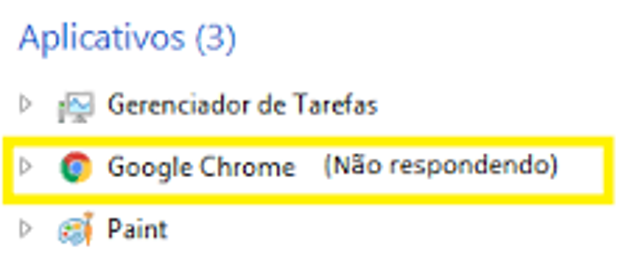
\includegraphics[width=0.4\textwidth, keepaspectratio]{../figs/cap03/omissaoprocesso.png}
		\end{figure}		
	\end{frame}
	
	\begin{frame}{Falha por omissão de comunicação}		
		\begin{figure}[hbtp]
		\centering
		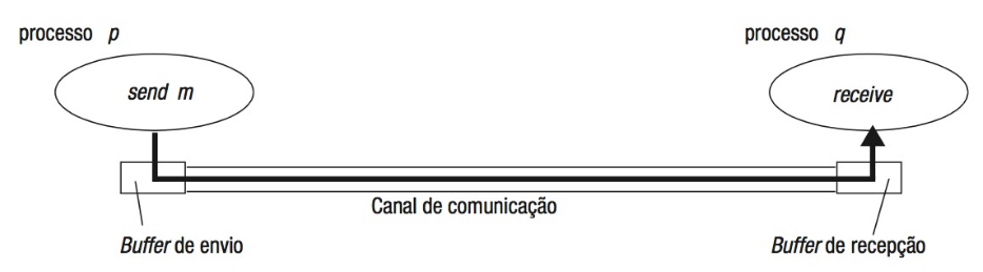
\includegraphics[width=0.85\textwidth, keepaspectratio]{../figs/cap03/omissaocomunicacao.png}
		\end{figure}	
	\end{frame}
	
	\begin{frame}{Falhas arbitrárias}
		\begin{itemize}
			\item Pior tipo de falha
			\begin{itemize}
				\item Atribuição incorreta de valores
				\item Corrupção de mensagens
				\item Envio de mensagens inexistentes
			\end{itemize}
		\end{itemize}
	\end{frame}
	
	\begin{frame}{Tipos de falhas}
		\begin{figure}[hbtp]
		\centering
		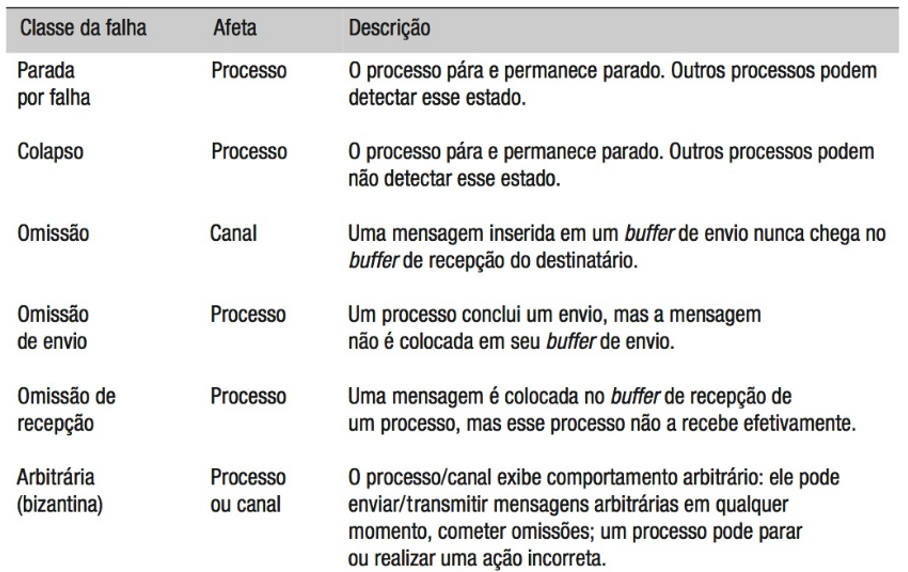
\includegraphics[width=0.80\textwidth, keepaspectratio]{../figs/cap03/falhas1.png}
		\end{figure}	
	\end{frame}
	
	
	\begin{frame}{Falhas de temporização}
		\begin{itemize}
			\item Afetam apenas sistemas síncronos
		\end{itemize}
		
		\begin{figure}[hbtp]
		\centering
		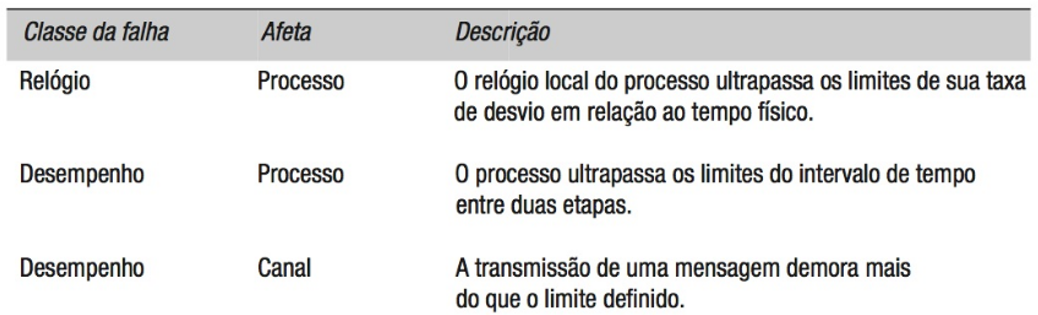
\includegraphics[width=0.85\textwidth, keepaspectratio]{../figs/cap03/falhas2.png}
		\end{figure}		
	\end{frame}
	

	\section{Modelo de Segurança}	
	
	\begin{frame}{Segurança}
	\begin{quote}
	\Large
	"A segurança de um sistema distribuído pode ser obtida tornando seguros os processos e os canais usados por suas interações e protegendo contra acesso não autorizado os objetos que encapsulam." – COULOURIS, 2013

	\end{quote}
	\end{frame}
	
	\begin{frame}{Onde aplicar segurança?}
		\begin{itemize}
			\item Processos
			\begin{itemize}
				\item Vulnerabilidades 
			\end{itemize}
			\vspace{1em}			
			\item Canais
			\begin{itemize}
				\item Sniffers
			\end{itemize}
			\vspace{1em}
			\item Objetos
			\begin{itemize}
				\item Uso não autorizado
			\end{itemize}
		\end{itemize}
	\end{frame}
	
	\begin{frame}{Proteção a objetos}
		\begin{itemize}
			\item Direitos de acesso
			\begin{itemize}
				\item Definem quem pode acessar determinado recurso
			\end{itemize}
		\end{itemize}
				
		\begin{figure}[hbtp]
		\centering
		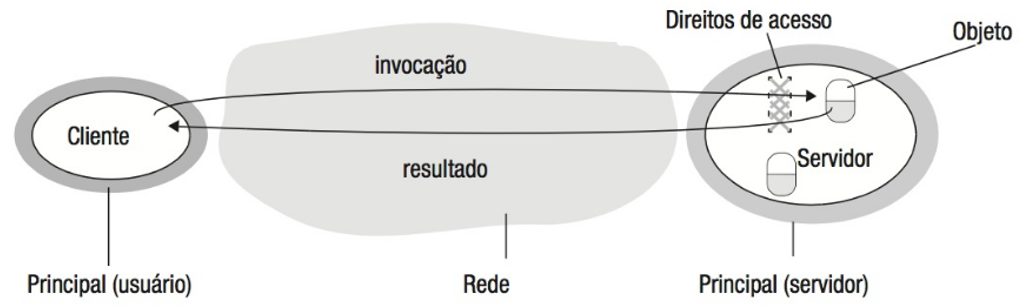
\includegraphics[width=0.85\textwidth, keepaspectratio]{../figs/cap03/protecaoobjeto.png}
		\end{figure}	
	\end{frame}
	
	\begin{frame}{Ameaças ao processo}
		\begin{itemize}
			\item Problemas de identificação 
			\begin{itemize}
				\item Roubo de senhas
				\item Roubo de informações
				\item Roubo de identidade
				\item Violação de direitos de acesso
				\item Páginas falsas

			\end{itemize}

		\end{itemize}
	\end{frame}
	
	\begin{frame}{Ameaças ao canal de comunicação}
		\begin{itemize}
			\item Alteração, cópia e/ou extração de mensagens de um canal de comunicação
		\end{itemize}
		
		\begin{figure}[hbtp]
		\centering
		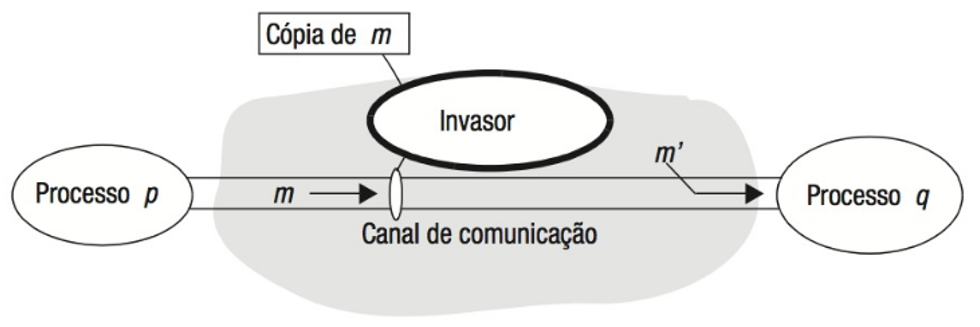
\includegraphics[width=0.85\textwidth, keepaspectratio]{../figs/cap03/ameacacanal.png}
		\end{figure}	
	\end{frame}
	
	\begin{frame}{Negação de serviço}
		\begin{itemize}
			\item Ataque para retardar ou impedir o acesso de usuários a um sistema
			\begin{itemize}
				\item Realização de múltiplas invocações 
				\item Envio incessante de mensagens
			\end{itemize}
			\vspace{1em}
			\item Causado por sobrecarga dos recursos físicos
			\begin{itemize}
				\item Processamento
				\item Largura de banda
				\item Memória
			\end{itemize}
		\end{itemize}
	\end{frame}
	
	\begin{frame}{Fornecendo segurança ao sistema}
		\begin{itemize}
			\item Criptografia
			\vspace{1em}
			\item Autenticação
			\vspace{1em}
			\item Canais seguros
		\end{itemize}
	\end{frame}
	
	\begin{frame}{Análise de segurança}
		\begin{itemize}
			\item Listar formas de ataque possíveis
			\begin{itemize}
				\item Rede
				\item Ambiente Físico
				\item Processos
			\end{itemize}
			\vspace{1em}
			\item Avaliar custo benefício das soluções de segurança
			\vspace{1em}
			\item Entender o RISCO HUMANO para o sistema
		\end{itemize}
	\end{frame}
		
	\begin{frame}{}
	\end{frame}	
\end{document}
